\documentclass[a4paper,12pt,twoside]{scrreprt}
% Autor der Vorlage: Klaus Rheinberger, FH Vorarlberg, 2017-02-20

% Pakete:
\usepackage[utf8]{inputenc}
\usepackage[T1]{fontenc} % Silbentrennung bei Sonderzeichen
\usepackage{graphicx} % Bilder einbinden
\usepackage{wrapfig} % Bilder positionieren
\usepackage[ngerman]{babel} % Deutsche Sprachanpassungen
\usepackage{minted} % Code Highlighting/Import
\usepackage{csquotes} % Anführungszeichen und Zitieren
\usepackage{acronym} % Abkürzungsverzeichnis
\usepackage[bindingoffset=8mm]{geometry} % Bindeverlust von 8mm einbeziehen
\usepackage{caption} % Abbildungslegenden
\usepackage{xcolor} % Farbige Hervorhebungen
\usepackage{setspace} % Zeilenabstand
\usepackage[style=authoryear,citestyle=authoryear,backend=biber]{biblatex} % Literaturverweise
\usepackage[
    linktocpage=true,
    pdfauthor={Dominic Luidold},
]{hyperref} % Links -> \href{https://www.wikibooks.org}{Wikibooks home}

% Einstellungen:
\captionsetup{format=hang, justification=raggedright}
\addbibresource{Zotero.bib}
\setcounter{secnumdepth}{4}
\setcounter{tocdepth}{4} % Tiefe der Gliederung im Inhaltsverzeichnis

% Custom Commands
\renewcommand{\listingscaption}{Quellcode}
\renewcommand\listoflistingscaption{Quellcodeverzeichnis}

% Dokumentenbeginn
\begin{document}
\onehalfspacing % Zeilenabstand 1,5

% Sperrvermerkseite
\thispagestyle{empty}

\section*{Sperrvermerk}
\label{sec:sperrvermerk}
Auf Wunsch der Firma Fusonic GmbH, im Auftrag der Viterma Handels GmbH, ist die vorliegende Arbeit bis zum [DATUM] für die öffentliche Nutzung zu sperren.

Veröffentlichung, Vervielfältigung und Einsichtnahme sind ohne ausdrückliche Genehmigung der oben genannten Firma und dem Verfasser nicht gestattet. Der Titel der Arbeit sowie das Kurzreferat/Abstract dürfen jedoch veröffentlicht werden.

\vspace{3cm}

\noindent Dornbirn, am [Datum] \hfill Unterschrift des Verfassers (Dominic Luidold)

\vspace{2cm}

\hfill Firmenstempel\hspace{2cm}

% Titelblatt:
% \newpage\mbox{}\newpage
\cleardoublepage   % force output to a right page
\thispagestyle{empty}
\begin{titlepage}
    \begin{flushright}
    
\includegraphics[width=0.4\linewidth]{images/Logo_FHV.jpg}
    \end{flushright}
    \begin{flushleft}
    \section*{[Titel der Arbeit]}
    \subsection*{[Untertitel der Arbeit]}
    \vspace{1cm}

    Bachelorarbeit I\\
    zur Erlangung des akademischen Grades
    \vspace{0.5cm}

    \textbf{Bachelor of Science in Engineering (BSc)}

    \vspace{1cm}
    Fachhochschule Vorarlberg\newline
    Informatik – Software and Information Engineering

    \vspace{0.5cm}

    Betreut von\newline
    Prof. (FH) Dipl. Inform. Thomas Feilhauer

    \vspace{0.5cm}

    Vorgelegt von\newline
    Dominic Luidold\newline
    Dornbirn, [Datum]
    \end{flushleft}
\end{titlepage}

% Widmung:
\newpage
\section*{Widmung}
\label{sec:widmung}
Trotz des Sperrvermerks, an der diese Arbeit gebunden ist, möchte ich es mir nicht nehmen lassen, den Personen einen Dank auszusprechen, die mich bei der Umsetzung und Realisierung meiner Bachelorarbeit I unterstützt haben.

\medskip

Zu Beginn möchte ich meinen Betreuern Thomas Feilhauer (Fachhochschule Vorarlberg) und Michael Zangerle (Fusonic GmbH) danken, die jederzeit ein offenes Ohr für Fragen, Anliegen und Unklarheiten hatten. Durch ihre fachliche Kompetenz, ihre langjährige Erfahrung sowie ihr Know-how konnte ich vieles lernen, das ich in mein weiteres Berufsleben mitnehmen kann.

\medskip

Als nächstes möchte ich meiner gesamten Familie danken, denen ich während des Schreibens dieser Arbeit wahrscheinlich mehr als nur einmal auf die Nerven gegangen bin. Nur durch die Tatkräftige Unterstützung mit Snacks, Süßigkeiten und dem besten Zimmerservice der Welt konnte ich so ungestört an der Bachelorarbeit schreiben. Ohne ihr Korrekturlesen wären zudem mehr Tippfehler vorhanden als mir lieb sind und ich auf meine Tastatur schieben kann.

\medskip

Zu guter Letzt möchte ich meine Arbeit all jenen widmen, die für die Gleichbehandlung und Gleichberechtigung aller kämpfen, sich für eine Sache einsetzen, die größer als sie selbst ist und für die sie teilweise sogar ihr Leben aufs Spiel setzen. Auch 2020 braucht es weltweit immer noch laute Stimmen - Stimmen, die sich nicht unterkriegen lassen.

\bigskip

\begin{quote}
    \begin{flushright}
        \textit{\enquote{The time is always right to do what is right.}}\\
        Dr. Martin Luther King Jr.
    \end{flushright}
\end{quote}

% Kurzreferat:
\newpage
\section*{Kurzreferat}
\label{sec:kurzreferat}

\subsection*{[Deutscher Titel Ihrer Arbeit]}

[Text des Kurzreferats]

% Abstract:
\newpage
\section*{Abstract}
\label{sec:abstract}

\subsection*{[English Title of your thesis]}

[text of the abstract]

% Vorwort:
\newpage
\section*{Vorwort}
\label{sec:vorwort}

Der Verfasser der vorliegenden Arbeit bekennt sich zu einer geschlechtergerechten Sprachverwendung.

Um die Lesbarkeit zu gewährleisten und zugunsten der Textökonomie werden die verwendeten Personen beziehungsweise Personengruppen fix männlich oder weiblich zugeordnet. Zum Beispiel wird immer \enquote{die Entwicklerin} und \enquote{der Benutzer} verwendet. Es wurde besonders darauf geachtet, stereotype Rollenbeschreibungen zu vermeiden. Die insgesamt eventuell dadurch hervorgerufene Irritation bei den Lesenden ist gewünscht und soll dazu beitragen, eine Bewusstheit für die bestehende, Frauen diskriminierende Sprachgewohnheit (generelle Verwendung der männlichen Begriffe für beide Geschlechter) zu wecken beziehungsweise zu stärken.

% Inhaltsverzeichnis:
\cleardoublepage % force output to a right page
\tableofcontents

\clearpage
\phantomsection
\addcontentsline{toc}{chapter}{Abbildungsverzeichnis}
\listoffigures

\clearpage
\phantomsection
\addcontentsline{toc}{chapter}{Quellcodeverzeichnis}
\listoflistings

\clearpage
\phantomsection
\addcontentsline{toc}{chapter}{Tabellenverzeichnis}
\listoftables

% Abkürzungsverzeichnis:
\clearpage
\phantomsection
\addcontentsline{toc}{chapter}{Abkürzungsverzeichnis}
\chapter*{Abkürzungsverzeichnis}
\begin{acronym}
 \acro{BLS}{Better Life System}
 \acro{CI}{Continuous Integration}
 \acro{CD}{Continuous Deployment}
 \acro{CQS}{Command Query Separation}
 \acro{CQRS}{Command Query Responsibility Segregation}
 \acro{CRUD}{Create, Read, Update, Delete}
 \acro{DTO}{Data Transfer Object}
 \acro{IDE}{Integrierte Entwicklungsumgebung}
 \acro{LTS}{Long Term Support}
 \acro{MVC}{Model View Controller}
\end{acronym}

\chapter{Einleitung}
\label{chap:einleitung}
Diese Bachelorarbeit verfolgt das Ziel, einen Einblick in die Implementierung und Erweiterung des bereits bestehenden Backend-Systems des \enquote{Better Life System} (kurz \enquote{BLS}) der Viterma Handels GmbH mit dem sogenannten \enquote{CQRS}-Pattern zu geben.

Das Better Life System - welches von Fusonic GmbH entwickelt wird und mittels einer Weboberfläche und gängigen Webbrowsern bedient werden kann - ermöglicht es Endkunden, mithilfe einer Handelsvertreterin der Firma Viterma (beziehungsweise mit einer Vertreterin eines ihrer Franchise-Partner) ein Badezimmer anhand der jeweiligen Bedürfnisse auszusuchen und zu konfigurieren, um sich schlussendlich ein entsprechendes Angebot dafür erstellen zu lassen.

\section{Arbeitgeber Fusonic GmbH}
\label{sec:arbeitgeber}
Die Fusonic GmbH hat ihren Firmensitz in Götzis, Vorarlberg, und besteht aus einem Team von aktuell mehr als 25 Angestellten, Softwareentwicklerinnen und Projektleiterinnen. Diese sind aufgeteilt in diverse kleinere Teams, die intern unter anderem \enquote{Duck-Team} beziehungsweise \enquote{Parrot-Team} genannt werden. Die Teams arbeiten dabei an jeweils eigenständigen Projekten und setzen diverse Technologien ein. Zu den verwendeten Technologien gehören unter anderem C\# mit .NET, PHP mit Symfony und JavaScript/TypeScript mit Angular. \parencite[vgl.]["Übersicht aller Technologien"]{fusonic_gmbh_web_2020} Während es  regelmäßigen Austausch unter den Teams gibt, besteht jedes aus Frontend- sowie Backend-Entwicklern, da die meisten Projekte - aufgrund der zugrundeliegenden Anwendungsfälle - aus einem Web-Frontend sowie serverseitgen Backend bestehen.

\section{Nutzung \& Umfeld des \enquote{Better Life System}}
\label{sec:nutzung-umfeld}
Die Hauptaufgabe des Better Life System liegt darin, als computergestütztes und plattformunabhängiges Tool, Vertreterinnen rund um die Viterma Handels GmbH bei der Konfiguration und Zusammenstellung eines Badezimmers - zusammen mit dem Endkunden (meist Haus- beziehungsweise Wohnungsbesitzer oder Hotels) - zu unterstützen und diesen Vorgang zu erleichtern. Das BLS wird des Weiteren dazu verwendet, aktuelle und abgeschlossene Angebote zu verwalten, Produkte, Produktinformationen und dazugehörige Preisaufschläge zu pflegen und Kundendaten abzulegen. Zudem dient es als Kontrollinstanz für in Auftrag gegebene Sanierungen, um sicherzustellen, dass alle benötigten Materialen und Teile in entsprechenden Mengen vorhanden und kompatibel sind.

Die Nutzung des BLS findet zu großen Teilen auf mobilen Rechnern beziehungsweise Laptops statt, die während der Beratung und Betreuung von Kunden zum Einsatz kommen. Da nicht immer gewährleistet werden kann, dass eine aufrechte Internetverbindung besteht, ist die Offline-Fähigkeit bei gleichbleibender Nutzung im Webbrowser ein wichtiger Bestandteil des Web-Frontends.

Aufgrund der Anforderungen der Viterma Handels GmbH, dass das Better Life System offline ebenso wie online verwendet werden kann, basiert das Frontend auf dem TypeScript Web-Framework Angular\footnote{\href{https://angular.io/}{Angular (https://angular.io)}}, welches solch eine Funktionalität ohne eine Installation oder zusätzliche Voraussetzungen am Endgerät unterstützt. Im Gegensatz zu weniger komplex gehaltenen Frontends - die primär Daten darstellen, die vom Backend eingehen - ist dieses beim BLS für einen Großteil der Ablauflogik, Berechnung von Preisen und Generierung von diversen PDFs zuständig. Das Frontend wird, da der Fokus dieser Arbeit auf der Entwicklung im Backend der Anwendung liegt, in weiterer Folge jedoch nicht genauer beleuchtet und als gegeben angenommen. Es kann davon ausgegangen werden, dass eingehende Anfragen an das Backend aus Benutzereingaben beziehungsweise zeitlich gesteuerten Events resultieren.

\pagebreak

Das Backend, welches alle API-Anfragen bearbeitet und als Schnittstelle zur Datenbank dient, ist in der Programmiersprache PHP geschrieben und verwendet das Framework Symfony\footnote{\href{https://symfony.com/}{Symfony (https://symfony.com)}} sowie diverse \enquote{Bundles}, die darauf aufbauen. Ein detaillierterer Überblick über den Aufbau, bisher angewandte Konzepte sowie technische Begebenheiten werden in Kapitel~\ref{chap:stand-technik} ab Seite \pageref{chap:stand-technik} behandelt.

\medskip

Während die Nutzung des Better Life System auf allen Plattformen - die einen modernen Webbrowser anbieten - möglich ist, findet die Entwicklung primär auf der Linux-Distribution  Ubuntu statt. Der Grund für diese Betriebssystemwahl ist damit zu erklären, dass sowohl die lokale Entwicklung als auch die Continuous Integration Umgebung (genutzt für automatisierte Tests) und das Continuous Deployment mittels Docker\footnote{\href{https://docker.com}{Docker (https://docker.com)}} Containern stattfindet. Für die Entwicklung im Backend-Bereich der Anwendung wird die IDE PhpStorm verwendet, während im Frontend auf Visual Studio Code gesetzt wird.

\section{Problemstellung}
\label{sec:problemstellung}
Die Entwicklung des BLS hat im Frühjahr 2017 begonnen und die Anwendung ist seit dem stetig weiterentwickelt worden. Über die Zeit haben sich entsprechend sowohl die Anforderungen und Wünsche des Kunden als auch die technischen Begebenheiten, Best Practices und Möglichkeiten verändert.

Die bisher bei der Umsetzung des Projekts verwendete Struktur sowie der Aufbau wurde stark an die empfohlene Herangehensweise von Symfony angelehnt und die Code-Basis entsprechend darauf ausgelegt \parencite[siehe dazu][\enquote{Use the Default Directory Structure}]{symfony_symfony_2020}. Durch wachsende Anforderungen und entsprechend benötigten Programmcode, der diese erfüllt, hat sich jedoch ein komplexes System ergeben, dessen \textit{Controller}, \textit{Entities}, \textit{Manager (Services)} und \textit{Data Transfer Objects (DTOs)} auf viele Verzeichnisse und Unterverzeichnisse verteilt sind. Die Abbildung~\ref{fig:ordnerstruktur} auf Seite \pageref{fig:ordnerstruktur} zeigt einen Ausschnitt von Ordnern die im Projekt vorkommen und jeweils alle Klassen ihrer Art beinhalten (im Verzeichnis \enquote{Controller} befinden sich, um ein Beispiel zu nennen, alle Controller des Projekts).

\begin{figure}[ht]
    \centering
    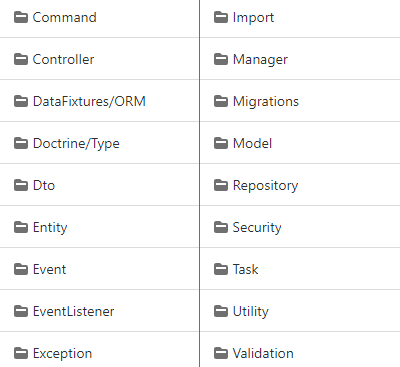
\includegraphics[scale=0.75]{images/bls_folder_structure.png}
    \caption{Teilausschnitt der BLS-Ordnerstruktur}
    \label{fig:ordnerstruktur}
\end{figure}

Durch die bisher gewählte Herangehensweise und den entsprechenden Aufbau hat sich jedoch ergeben, dass eine logische Gruppierung beziehungsweise Kapselung von zusammengehörenden Klassen, Controllern, Managern etc. eines API Endpunkts nur schwer möglich ist. Das hat zur Folge, dass das System an manchen Stellen sehr komplex aufgebaut ist und externe Personen eine gewisse Zeit brauchen, um sich mit internen Abläufen vertraut machen zu können. Neben der Verständlichkeit ist dadurch in weiterer Folge auch die Wartbarkeit und einfache Erweiterbarkeit im Falle von neuen Funktionalitäten nicht im vollen Ausmaß gegeben. Das Testen einzelner Bestandteile mittels sogenannter \textit{Unit Tests} findet im Moment nur an wenigen Stellen statt. Primär wird beim Better Life System auf \textit{Integration Tests} gesetzt, die im Problemfall jedoch nur grundsätzlich darauf hindeuten können, wo ein Fehler aufgetreten ist.

Da sich die Anforderungen an das Backend auch in Zukunft noch weiterentwickeln können und eine Skalierung der Infrastruktur beziehungsweise Abspaltung einzelner Teile (in sogenannte Microservices) nicht ausgeschlossen werden kann, bedarf es Möglichkeiten, dies möglichst effektiv und ohne großen, zusätzlichen Aufwand umsetzen zu können. Die von Symfony empfohlene Herangehensweise kann dies dabei nur bedingt unterstützen, was auch in diesem Fall einen limitierenden Faktor darstellt.

\section{Anforderungen}
\label{sec:anforderungen}
Die in Abschnitt~\ref{sec:problemstellung} angeführten Umstände und den daraus resultierenden Herangehensweisen, die nicht mehr in vollem Maße zufriedenstellend sind, führen zu neuen Anforderungen an das Better Life System. Diese sollen entsprechend umgesetzt werden, um ein zukunftssicheres Backend für die gesamte Anwendung garantieren zu können und die Entwicklung neuer sowie bestehender Funktionalitäten zu erleichtern und zu vereinheitlichen.

\medskip

Zum Start des Berufspraktikums Anfang Juli 2020 stand bereits fest, dass in weiterer Folge das CQRS-Pattern (was für \textit{Command Query Responsibility Segregation} steht) zum Einsatz kommen wird. Andere Projekte der Fusonic GmbH, die primär auf C\# und .NET basieren, haben bereits gute Erfahrungen damit gemacht und gehen deshalb davon aus, dass der Einsatz Patterns die Qualität der bestehenden Code-Basis verbessern wird.

\medskip

Die Anforderungen, die im Zuge des Berufspraktikums und folglich dieser Bachelorarbeit zu erfüllen sind, bestehen darin, das aktuell bestehende System, neben dem \enquote{Tagesgeschäft} (sprich Bugfixes, Feature Requests etc.), laufend umzustellen und neue Funktionalitäten entsprechend mit der neuen Struktur und dem Pattern umzusetzen.

\section{Zielsetzung}
\label{sec:zielsetzung}
Die in den Abschnitten~\ref{sec:problemstellung} und \ref{sec:anforderungen} angeführten Punkte ergeben folgende Ziele, die im Verlauf des Berufspraktikums - so weit wie möglich - umzusetzen sind.

\smallskip

\noindent
Als Ziele einzustufen sind:
\begin{itemize}
    \item Vorbereitung der bestehenden Infrastruktur auf CQRS in Zusammenarbeit mit Mitarbeitern der Fusonic GmbH
    \item Umstellung der bestehenden API Endpunkte auf CQRS bei Beibehaltung von möglichst viel Programmlogik
    \item Umsetzung neuer Funktionalitäten mittels CQRS
    \item Weiterhin Abwickeln des Tagesgeschäftes
\end{itemize}

\chapter{Stand der Technik}
\label{chap:stand-technik}
Das folgende Kapitel gibt einen Überblick über den aktuellen Stand des Backends des Better Life System, dessen technischem Aufbau und dem zugrundeliegenden Konzept. Anschließend wird die von Symfony vorgeschlagene Architektur beleuchtet und auf das zukünftig eingesetzte CQRS-Pattern eingegangen. Am Ende des Kapitels werden die gängige Schichtenarchitektur und CQRS gegenübergestellt und Vor- sowie Nachteile aufgezeigt.

\section{Aufbau des Backends}
\label{sec:aufbau-backend}
Das Backend des BLS basiert auf der Programmiersprache PHP und setzt hierbei auf die zum aktuellen Zeitpunkt (Stand August 2020) neueste Version \textit{PHP 7.4}. Zur Verwaltung benötigter Abhängigkeiten kommt das Paketverwaltungssystem Composer\footnote{\href{https://getcomposer.org}{Composer (https://getcomposer.org)}} zum Einsatz, welches alle benötigten Symfony Bundles und anderweitige Packages - sowohl im Produktivsystem als auch während der Entwicklung - zur lokalen Installation sowie Nutzung zur Verfügung stellt.

Als Grundgerüst für das Backend dient das PHP-Framework Symfony in der LTS-Version \textit{4.4}, wobei zum Zeitpunkt des Verfassens dieser Arbeit Vorbereitungen für einen Umstieg auf Version \textit{5.x} getroffen werden. Das Backend dient als Schnittstelle zwischen dem Angular-Frontend und einem Datenspeicher, wobei hierfür eine relationale Datenbank auf Basis von MySQL eingesetzt wird. Um von Symfony aus auf die Datenbank zugreifen zu können, wird Doctrine\footnote{\href{https://www.doctrine-project.org}{Doctrine (https://www.doctrine-project.org)}} eingesetzt, welches ein objektrelationales Mapping vornimmt und in der Anwendung zur Verfügung stellt.

Der grundsätzliche Aufbau des Symfony Backends entspricht aktuell der empfohlenen Vorgehensweise laut Symfony Dokumentation und wird im nachfolgenden Abschnitt~\ref{sec:standard-schichtenarchitektur} erläutert.

\section{Gängige Schichtenarchitektur}
\label{sec:standard-schichtenarchitektur}

Symfony ist ein Webframework, welches aus vielen verschiedenen Komponenten und Bundles besteht, die alle unabhängig voneinander entwickelt werden. In Summe ergeben diese die Grundlage für eine Webapplikation auf Basis von PHP und werden auch von anderen Frameworks verwendet (beispielsweise Laravel\footnote{\href{https://laravel.com}{Laravel (https://laravel.com)}}, welches auf diversen Symfony-Komponenten basiert). Symfony orientiert sich dabei an der weit verbreiteten \textit{Model View Controller} Architektur (kurz \textit{MVC}) und bietet mittels flexiblem URI Routing, Session beziehungsweise Security Management und Logging unterstützende Funktionalitäten. \parencite[Vgl.][]{tutorials_point_i_pvt_ltd_symfony_nodate-1}

\subsection{Empfohlener Ansatz}
\label{sub-sec:empfohlener-ansatz}
Symfony selbst gibt in der eigenen Dokumentation keine verpflichtenden Vorgaben an, wie genau man eine Applikation beziehungsweise Anwendung umsetzen soll. \parencite[Vgl.][]{symfony_symfony_2020} Der Quellcode~\ref{code:symfony-project-structure} auf Seite \pageref{code:symfony-project-structure} zeigt den empfohlenen Aufbau einer Anwendung, bei der man die Anlehnung an das MVC-Pattern jedoch gut erkennen kann:

\begin{itemize}
    \item \textbf{Model:} Dem Model entsprechen die im \textit{Entity}-Verzeichnis abgelegten Klassen. Diese beinhalten das objektrelationale Mapping und können zusätzliche, domänenspezifische Funktionalitäten zur Verfügung stellen. Die Klassen, die im \textit{Repository}-Verzeichnis zu finden sind, stellen den Zugriff auf die Datenbank her und befüllen die Entities bzw. Models mit Daten. \parencite[Vgl.][]{tutorials_point_i_pvt_ltd_symfony_nodate}
    \item \textbf{View:} Im Falle der hier angenommenen Standardstruktur, wird der View-Teil mittels der Template Engine \textit{Twig} im gleichnamigen Verzeichnis abgehandelt. Im Falle des BLS ist dies mittels Data Transfer Objects gelöst, die bei den jeweiligen API Endpunkten als  serialisierte JSON-Response zurückgegeben werden. \parencite[Vgl.][]{tutorials_point_i_pvt_ltd_symfony_nodate}
    \item \textbf{Controller:} Die von der Namensgebung her am leichtesten zu erkennende Ähnlichkeit stellt das \textit{Controller}-Verzeichnis dar. Die darin vorhandenen Klassen werden verwendet, um eingehende Requests zu mappen. Diese Controller-Klassen sollten jedoch nur wenige Zeilen Code beinhalten, um Berechtigungen zu überprüfen sowie die Response zu erstellen. Die tatsächliche Businesslogik wird in separate Klassen aufgeteilt, die vom Controller aufgerufen werden, um diese möglichst zu entkoppeln. \parencite[Vgl.][]{symfony_symfony_2020} Beim BLS liegt die Anwendungslogik beispielsweise in einem \textit{Manager}-Verzeichnis.
\end{itemize}

\begin{listing}[ht]
    \inputminted[fontsize=\footnotesize,linenos]{text}{code/symfony_directory_structure.txt}
    \caption[Von Symfony empfohlener Projektaufbau]{Von Symfony empfohlener Projektaufbau. Quelle: \cite[]{symfony_symfony_2020}}
    \label{code:symfony-project-structure}
\end{listing}

\subsection{Funktionsweise}
\label{sub-sec:standard-funktionsweise}
Die Funktionsweise der von Symfony vorgeschlagenen Architektur kann, unter Bezugnahme auf die in Abschnitt~\ref{sub-sec:empfohlener-ansatz} beschriebenen Prinzipien, mithilfe der Abbildung~\ref{fig:single-model-fowler} genauer beleuchtet werden.

\smallskip

Im Zuge der Entwicklung einer Webapplikation mit entsprechendem Backend oder einer API  wird oftmals auf CRUD beziehungsweise einen CRUD-ähnlichen Aufbau gesetzt. Die Nutzung eines einzelnen Models, dem jeweiligen DTO (sofern vorhanden) sowie der dazugehörenden Businesslogik ist dabei ein einfacher Weg, um schnell und anfangs unkompliziert Funktionalitäten für die CRUD Anwendungsfälle umsetzen zu können. Auch bei weiterführenden Nutzungsfällen, bei denen beispielsweise mehrere Models zusammengeführt und entsprechend validiert werden müssen, wird die bestehende Logik herangezogen und keine spezifische Auftrennung von ausgeführten Aktionen vorgenommen. Dadurch entsteht jedoch eine Vermischung von lesenden und schreibenden Zugriffen in der Anwendungslogik sowie der Funktionalitäten der entsprechenden Models. \parencite[Vgl.][]{fowler_cqrs_2011} Die Abbildung stellt diesen Umstand anschaulich im hellgrau hinterlegten Rechteck \enquote{Application} dar:

\begin{figure}[ht]
    \centering
    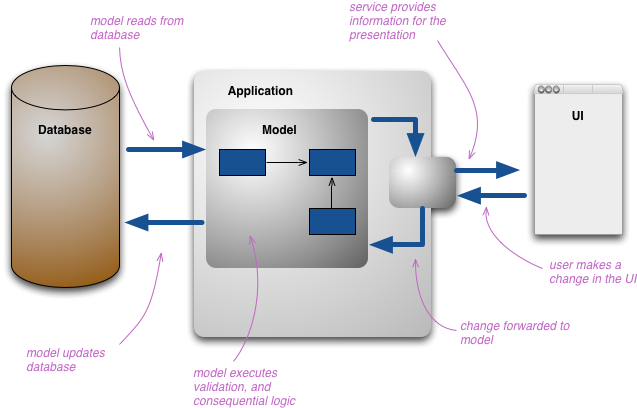
\includegraphics[scale=0.55]{images/fowler_single_model.png}
    \caption[Aufbau einer gängigen Schichtenarchitektur]{Aufbau einer gängigen Schichtenarchitektur.\\Quelle: \cite{fowler_cqrs_2011}}
    \label{fig:single-model-fowler}
\end{figure}

\section{CQRS Pattern}
\label{sec:cqrs-pattern}
Das Command Query Responsibility Segregation Pattern (nachfolgend CQRS genannt) soll als Grundlage für die zukünftige Struktur des Better Life System dienen. Die Entscheidung für den Wechsel auf dieses Pattern beziehungsweise die zugrundeliegende Architektur basiert primär auf Erfahrungswerten, die Fusonic GmbH bei anderen Projekten sammeln konnte. Der Einsatz dieses Patterns soll die im Kapitel~\ref{chap:einleitung} angesprochenen Problemstellungen in Angriff nehmen und die Komplexität, Verständlichkeit, Testbarkeit und Erweiterbarkeit des Systems langfristig verbessern.

Die bisherigen Erfahrungen, die Fusonic mit dieser Herangehensweise gemacht hat, basieren auf C\# und .NET Core Projekten. Ein entsprechender Einsatz mit der Programmiersprache PHP und dem Framework Symfony wurde bisher nur konzeptionell durchgeplant und findet damit erstmalig Einzug in ein Kundenprojekt.

\subsection{Grundlagen von CQRS}
\label{sub-sec:cqrs-grundlagen}
Um über das CQRS-Pattern sprechen zu können, werden einige grundlegende Begrifflichkeiten sowie Konzepte benötigt, die im weiteren Verlauf dessen Ursprung definieren und Verständnis schaffen sollen.

CQRS, beziehungsweise die Terme \textit{Command} und \textit{Query}, beziehen sich auf das Prinzip der \textit{Command Query Separation} (kurz \textit{CQS}). \parencite[Vgl.][]{young_cqrs_2010} CQS definiert auf der einen Seite lesende und auf der anderen Seite schreibende Aktionen in einem System, die voneinander getrennt sind und unterschiedlich agieren sowie verschiedene Resultate als Folge haben:

\begin{itemize}
    \item Lesende Aktionen, sogenannte \textbf{Queries}, greifen auf Daten in einem System zu und liefern diese bei einem Aufruf als Ergebnis zurück. Durch das Ausführen der Aktion wird der Zustand eines Objekts oder dem System im Ganzen nicht verändert. \parencite[Vgl.][]{fowler_commandqueryseparation_2005}
    \item Schreibende Aktionen, sogenannte \textbf{Commands}, verändern Daten in einem System, führen jedoch zu keinem Rückgabewert. Durch das Ausführen der Aktion wird der Zustand eines Objekts oder dem System im Ganzen bleibend verändert. \parencite[Vgl.][]{fowler_commandqueryseparation_2005}
\end{itemize}

\noindent
Fowler beschreibt den Vorteil dieser Aufteilung damit, dass Methoden, die den Zustand eines Objekts oder Systems verändern, von denen logisch getrennt werden können, die nur lesend darauf zugreifen. Queries können dadurch \enquote{gefahrlos} und in beliebiger Reihenfolge an jeder Stelle in einer Anwendung eingesetzt werden während dies bei Commands nicht gegeben ist. \parencite[Vgl.][]{fowler_commandqueryseparation_2005}

\subsection{Funktionsweise von CQRS}
\label{sub-sec:cqrs-funktionsweise}
Die Funktionsweise des CQRS Konzepts basiert, wie im Abschnitt~\ref{sub-sec:cqrs-grundlagen} beschrieben, auf dem Einsatz von Commands und Queries. Durch deren Einsatz wird eine effektive Aufteilung in zwei separate und optimalerweise unabhängige Modelle erzielt, wodurch zum einen ein Fokus auf die jeweilige Verantwortlichkeit des Modells gelegt werden kann und zum anderen die übermäßige Optimierung hin zu einer Datenbank wegfällt. Dadurch rückt die Anwendungs- beziehungsweise Businesslogik deutlich mehr in den Vordergrund und kann entsprechend besser ausgebaut und getestet werden. \parencite[Vgl.][]{heimeshoff_cqrs_2013}

\medskip

Anhand der Abbildung~\ref{fig:cqrs-fowler} auf Seite \pageref{fig:cqrs-fowler} wird verdeutlicht, wie der Ablauf in einem auf CQRS basierenden System abläuft:

\textbf{Ändern von Daten:} Eine vom Benutzer ausgelöste Änderung der Daten (im Falle des BLS durch eine Aktion im Angular-Frontend) führt dazu, dass diese an ein Command Model (oftmals vergleichbar mit einem Domänenmodell auf Basis des Domain-Driven Designs \parencite[vgl.][]{heimeshoff_cqrs_2013}) weitergeleitet wird. Dieses beinhaltet domänenspezifische Logik, Validierung und gegebenenfalls weitere benötigte Funktionalitäten. Das Command Model, dass die Integrität der eingehenden Daten sichergestellt hat, persistiert diese abschließend in der Datenbank und schließt die Aktion (den Command) somit ohne Rückgabewert ab. \parencite[Vgl.][]{fowler_cqrs_2011}

\textbf{Abfragen von Daten:} Ein Abfragen der Daten (ebenfalls durch das Frontend ausgelöst) führt dazu, dass diese von der Datenbank geladen und mittels des Query Models (in manchen Fällen auch mehrer) im entsprechenden Format serialisert werden. Das Query Model schließt die Aktion damit ab, dass die serialisierten Daten nach außen als Rückgabewert(e) zurückgegeben werden. \parencite[Vgl.][]{heimeshoff_cqrs_2013}

\vspace{0.5cm}

\begin{figure}[ht]
    \centering
    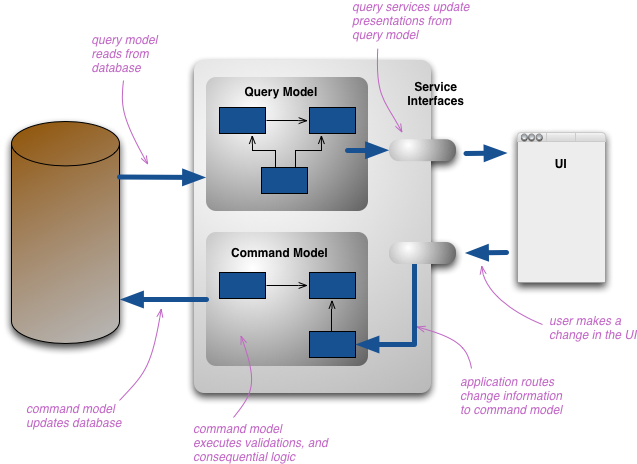
\includegraphics[scale=0.6]{images/cqrs_fowler.png}
    \caption[Schematischer Aufbau eines auf CQRS basierenden Systems]{Schematischer Aufbau eines auf CQRS basierenden Systems.\\Quelle: \cite{fowler_cqrs_2011}}
    \label{fig:cqrs-fowler}
\end{figure}

\section{Vergleich Schichtenarchitektur und CQRS}
\label{sec:vergleich-schichten-cqrs}

\colorbox{yellow}{TODO}

% Literaturverzeichnis:
\clearpage
\phantomsection
\addcontentsline{toc}{chapter}{Literaturverzeichnis}
\printbibliography

\chapter*{[evtl. Anhang]}  % evtl. ersetzen mit \chapter*{Anhang}
\addcontentsline{toc}{chapter}{[evtl. Anhang]}   % evtl. ersetzen mit \addcontentsline{toc}{chapter}{Anhang}
Formatvorlage für den Fließtext.

\chapter*{Eidesstattliche Erklärung}
\addcontentsline{toc}{chapter}{Eidesstattliche Erklärung}
Ich erkläre hiermit an Eides statt, dass ich die vorliegende Bachelorarbeit I selbstständig und ohne Benutzung anderer als der angegebenen Hilfsmittel angefertigt habe. Die aus fremden Quellen direkt oder indirekt übernommenen Stellen sind als solche kenntlich gemacht. Die Arbeit wurde bisher weder in gleicher noch in ähnlicher Form einer anderen Prüfungsbehörde vorgelegt und auch noch nicht veröffentlicht.

\vspace{3cm}
\noindent
Dornbirn, am [Datum]\hfill Dominic Luidold

\end{document}
